% !TEX root = ../../../main.tex
\begin{samepage}
\section{Rank}
\label{sec:linear-algebra-i:rank}

% Sources: supplied lecture photos and September 24 slides 3--17.
\begin{definition}
  The rank of a linear map is the dimension of its image:
  \[
    \operatorname{rank}L=\dim\operatorname{im}L.
  \]
  Its nullity, introduced in \autoref{sec:linear-algebra-i:kernel},
  is \(\operatorname{nullity}L=\dim\ker L\).
\end{definition}
\end{samepage}

% Source: the author's additional rank notes, September 30, 2026.
\subsection{Rank of a matrix}

Let \(M\in\mathbb F^{m\times n}\), with \(m\) rows and \(n\) columns.
It represents the linear map \(x\mapsto Mx\) from \(\mathbb F^n\)
to \(\mathbb F^m\). If its columns are \(c_1,\ldots,c_n\), then
\[
  \operatorname{im}M=\operatorname{span}\{c_1,\ldots,c_n\}.
\]
Thus \(\operatorname{rank}M\) is the maximum number of linearly
independent columns of \(M\). Since there are \(n\) columns and each
belongs to \(\mathbb F^m\),
\[
  0\leq\operatorname{rank}M\leq\min(m,n).
\]

% The author requested explicit rank/nullity bounds on October 1, 2026.
Both rank and nullity are nonnegative integers because they are dimensions.
The kernel of \(M\) is a subspace of \(\mathbb F^n\), so
\[
  0\leq\operatorname{nullity}M\leq n.
\]
Here \(n\) is the number of columns, the dimension of the domain.
The rank--nullity theorem (\autoref{thm:linear-algebra-i:rank-nullity})
gives
\[
  \operatorname{nullity}M=n-\operatorname{rank}M.
\]
Combining this identity with the rank bound yields the sharper range
\[
  \max(0,n-m)\leq\operatorname{nullity}M\leq n.
\]
Thus rank and nullity cannot be chosen independently; their sum is \(n\).

Rank measures the non-degeneracy of a system of linear equations
\(Mx=b\) by counting its independent output directions. The matrix
has \emph{full rank} when its rank equals \(\min(m,n)\); a smaller
rank reflects additional linear dependencies. The value of \(b\)
still determines whether the system is consistent, through the
condition \(b\in\operatorname{im}M\).

\subsection{Examples in Euclidean spaces}

\begin{example}
  The inclusion \(Z:\R^2\to\R^3\), \(Z(x,y)=(x,y,0)\), has matrix
  \[
    \begin{bmatrix}1&0\\0&1\\0&0\end{bmatrix}.
  \]
  Its kernel is \(\{0\}\), and its image is the plane
  \(\{(x,y,0):x,y\in\R\}\), with basis
  \(\{(1,0,0),(0,1,0)\}\). Thus its nullity is \(0\) since the zero vector is not linearly independent and therefore cannot be a basis and its rank is \(2\).
\end{example}

\begin{example}
  For \(W:\R^2\to\R^3\), \(W(x,y)=(y,0,0)\), the matrix is
  \[
    \begin{bmatrix}0&1\\0&0\\0&0\end{bmatrix}.
  \]
  The kernel is \(\{(x,0):x\in\R\}\), with basis \(\{(1,0)\}\).
  The image is \(\{(y,0,0):y\in\R\}\), with basis \(\{(1,0,0)\}\).
  Hence its nullity is \(1\) and its rank is \(1\).
\end{example}

\begin{example}
  The zero map \(U:\R^2\to\R^3\) has matrix
  \[
    \begin{bmatrix}0&0\\0&0\\0&0\end{bmatrix},
  \]
  kernel \(\R^2\), and image \(\{(0,0,0)\}\). Its nullity is \(2\)
  and its rank is \(0\).
\end{example}

\begin{example}
  For \(U:\R^3\to\R^2\), \(U(x,y,z)=(y,z)\), the matrix is
  \[
    \begin{bmatrix}0&1&0\\0&0&1\end{bmatrix}.
  \]
  The kernel is \(\{(x,0,0):x\in\R\}\), with basis \(\{(1,0,0)\}\),
  and the image is \(\R^2\). Its nullity is \(1\) and its rank is \(2\).
\end{example}

\begin{example}
  For \(U:\R^3\to\R^2\), \(U(x,y,z)=(z,0)\), the matrix is
  \[
    \begin{bmatrix}0&0&1\\0&0&0\end{bmatrix}.
  \]
  The kernel is \(\{(x,y,0):x,y\in\R\}\), with basis
  \(\{(1,0,0),(0,1,0)\}\). The image is \(\{(z,0):z\in\R\}\),
  with basis \(\{(1,0)\}\). Its nullity is \(2\) and its rank is \(1\).
\end{example}

\begin{example}
  The zero map \(U:\R^3\to\R^2\) has matrix
  \[
    \begin{bmatrix}0&0&0\\0&0&0\end{bmatrix},
  \]
  kernel \(\R^3\), and image \(\{(0,0)\}\). Its nullity is \(3\)
  and its rank is \(0\).
\end{example}

\subsection{Adapted bases and rank--nullity}

The following lemma supplies a basis adapted to the kernel and image.

\begin{lemma}
  \label{thm:linear-algebra-i:adapted-basis}
  Let \(L:V\to W\) be a linear map between finite-dimensional vector
  spaces, with \(\dim V=m\) and \(\dim\ker L=k\). There is a basis
  \[
    (e_1,\ldots,e_k,e_{k+1},\ldots,e_m)
  \]
  of \(V\) such that \((e_1,\ldots,e_k)\) is a basis of \(\ker L\) and
  \((L(e_{k+1}),\ldots,L(e_m))\) is a basis of \(\operatorname{im}L\).
  If \(k=0\), the images of any basis of \(V\) form a basis of the image.
\end{lemma}
% Author review: September 24 slide 11 asserts this fact but does not prove
% basis extension or the spanning and independence of the remaining images.
% The earlier author notes also leave that verification open. The lemma
% remains a stated result; its missing proof has not been manufactured.

\begin{theorem}[Rank--nullity]
  \label{thm:linear-algebra-i:rank-nullity}
  For a linear map \(L:V\to W\) between finite-dimensional vector spaces,
  \[
    \operatorname{rank}L+\operatorname{nullity}L=\dim V.
  \]
\end{theorem}

\begin{proof}
  Set \(m=\dim V\) and \(k=\dim\ker L\). By
  \autoref{thm:linear-algebra-i:adapted-basis}, the image has a basis
  consisting of \(m-k\) vectors. Consequently,
  \[
    \dim\ker L+\operatorname{rank}L=k+(m-k)=m=\dim V.
  \]
\end{proof}

The following exercises apply these ideas.

% Source: MA-GY7033 Fall 2026 Homework 4.pdf, p. 1, Problem 1.
\begin{exercise}
  \label{ex:hw04:kernel-image-and-rank}
  \solutionlink{hw04:kernel-image-and-rank}
  Let \(T:\R^4\to\R^3\) be the linear map given by
  \[
    A=\begin{bmatrix}
      1&2&0&1\\
      0&1&1&1\\
      1&3&1&2
    \end{bmatrix}.
  \]
  \begin{enumerate}[(a)][2]
    \item Find \(\ker T\) and give a basis for it.
    \item Find \(\operatorname{im}T\) and give a basis for it.
    \item Compute the nullity and rank of \(T\), and verify the
      rank-nullity theorem.
    \item Determine whether \(T\) is injective and whether it is
      surjective. Justify both answers.
  \end{enumerate}
\end{exercise}


\subsection{Isomorphisms}

Recall the distinction between injectivity, surjectivity, and bijectivity
in \autoref{sec:appendix:map-properties}.
A linear map is an \emph{isomorphism} if it is injective and surjective.
The kernel and image criteria give
\[
  L\text{ is an isomorphism}
    \quad\Longleftrightarrow\quad
  \dim\ker L=0\text{ and }\operatorname{rank}L=\dim W.
\]
Rank--nullity then implies \(\dim V=\dim W\). Equivalently, \(L\) is an
isomorphism precisely when
\[
  \dim V=\dim W=\operatorname{rank}L,\qquad \dim\ker L=0.
\]
Another equivalent criterion is
\[
  L\text{ is bijective}
    \quad\Longleftrightarrow\quad
  \dim V=\dim W\text{ and }\dim\ker L=0.
\]

% Source: MA-GY7033 Fall 2026 Homework 4.pdf, p. 1, Problem 2.
\begin{exercise}
  \label{ex:hw04:rank-nullity}
  \solutionlink{hw04:rank-nullity}
  Answer each question using the rank-nullity theorem.
  \begin{enumerate}[(a)][2]
    \item Suppose \(L:V\to W\), where \(\dim V=7\), \(\dim W=5\),
      and \(\dim\ker L=3\). Find \(\operatorname{rank}L\).
      Is \(L\) injective? Is it surjective?
    \item Prove that every injective linear map \(T:\R^4\to\R^4\)
      is an isomorphism.
    \item Prove that no linear map from \(\R^6\) to \(\R^4\)
      can be injective.
    \item Prove that no linear map from \(\R^3\) to \(\R^5\)
      can be surjective.
  \end{enumerate}
\end{exercise}


\autoref{fig:linear-algebra-i:rank-map-criteria} summarizes the
rank and nullity tests for a linear map between finite-dimensional spaces.
The dimension inequalities are necessary consequences of these tests;
the sizes of the domain and codomain alone do not decide injectivity
or surjectivity. A bijective map satisfies both sets of criteria.

\begin{figure*}[htbp]
  \centering
  % Original schematic summary requested by the author, September 30, 2026.
% Numerical criteria assume finite-dimensional V and W.
% Circles show set containment; their radii do not encode dimensions.
\begin{tikzpicture}[
  x=1mm,y=1mm,font=\footnotesize,line width=0.45pt,
  every node/.style={inner sep=2pt},
  map arrow/.style={line width=0.35pt,-{Latex[length=1.6mm,width=1.1mm]}},
  criterion/.style={anchor=west,align=left}
]
  \node at (76,43) {Finite-dimensional \(L:V\to W\)};
  \node at (76,35)
    {\(\operatorname{rank}L+\operatorname{nullity}L=\dim V\)};

  % Injective: only zero lies in the kernel; the image can be proper.
  \begin{scope}
    \draw (14,0) circle[radius=12mm];
    \draw (56,0) circle[radius=12mm];
    \filldraw[fill=black!15] (56,0) circle[radius=9mm];
    \node at (14,16) {\(V\)};
    \node at (56,16) {\(W\)};
    \node at (14,-18) {\(\ker L=\{0_V\}\)};
    \node at (56,-18) {\(\operatorname{im}L\subseteq W\)};
    \draw[map arrow] (20,4)
      .. controls (34,10) and (45,10) .. (60,4);
    \draw[map arrow,dashed] (12,-3) -- (52,-3);
    \foreach \point in {(20,4),(60,4),(12,-3),(52,-3)}
      \fill \point circle[radius=1.6pt];
    \node at (57,-3) {\(0_W\)};

    \node[criterion] at (79,16) {\textbf{Injective}};
    \node[criterion] at (79,3)
      {\(\operatorname{rank}L=\dim V
        \ \Longleftrightarrow\ \operatorname{nullity}L=0\)};
    \node[criterion] at (79,-9)
      {Necessarily \(\dim V\leq\dim W\)};
  \end{scope}

  \draw[black!30] (0,-25) -- (153,-25);

  % Surjective: the entire codomain is the image; the kernel can be nonzero.
  \begin{scope}[yshift=-47mm]
    \draw (14,0) circle[radius=12mm];
    \filldraw[fill=black!35] (11,-2) circle[radius=6mm];
    \filldraw[fill=black!15] (56,0) circle[radius=12mm];
    \node at (14,16) {\(V\)};
    \node at (56,16) {\(W\)};
    \node at (14,-18) {\(\ker L\)};
    \node at (56,-18) {\(\operatorname{im}L=W\)};
    \draw[map arrow] (20,4)
      .. controls (34,10) and (45,10) .. (60,4);
    \draw[map arrow,dashed] (11,1)
      .. controls (28,1) and (40,-1) .. (52,-3);
    \draw[map arrow,dashed] (11,-2)
      .. controls (28,-7) and (40,-7) .. (52,-3);
    \foreach \point in {(20,4),(60,4),(11,1),(11,-2),(52,-3)}
      \fill \point circle[radius=1.6pt];
    \node at (57,-3) {\(0_W\)};

    \node[criterion] at (79,16) {\textbf{Surjective}};
    \node[criterion] at (79,3) {\(\operatorname{rank}L=\dim W\)};
    \node[criterion] at (79,-5)
      {\(\operatorname{nullity}L=\dim V-\dim W\)};
    \node[criterion] at (79,-15)
      {Necessarily \(\dim V\geq\dim W\)};
  \end{scope}

  \draw[black!30] (0,-72) -- (153,-72);

  % Bijective: zero kernel and image equal to the codomain.
  \begin{scope}[yshift=-94mm]
    \draw (14,0) circle[radius=12mm];
    \filldraw[fill=black!15] (56,0) circle[radius=12mm];
    \node at (14,16) {\(V\)};
    \node at (56,16) {\(W\)};
    \node at (14,-18) {\(\ker L=\{0_V\}\)};
    \node at (56,-18) {\(\operatorname{im}L=W\)};
    \draw[map arrow] (20,4)
      .. controls (34,10) and (45,10) .. (60,4);
    \draw[map arrow,dashed] (12,-3) -- (52,-3);
    \foreach \point in {(20,4),(60,4),(12,-3),(52,-3)}
      \fill \point circle[radius=1.6pt];
    \node at (57,-3) {\(0_W\)};

    \node[criterion] at (79,16) {\textbf{Bijective}};
    \node[criterion] at (79,3)
      {\(\operatorname{rank}L=\dim V=\dim W\)};
    \node[criterion] at (79,-5) {\(\operatorname{nullity}L=0\)};
    \node[criterion] at (79,-15) {Both injective and surjective};
  \end{scope}
\end{tikzpicture}

  \caption[Finite-dimensional map criteria.]{Finite-dimensional map criteria. Light gray shows the image;
    dark gray shows a nonzero kernel. Dashed paths map to zero.
    The first two sketches illustrate non-bijective possibilities.
    Circle sizes do not encode dimensions.}
  \label{fig:linear-algebra-i:rank-map-criteria}
\end{figure*}

\subsection{A matrix adapted to the kernel and image}

% The author requested motivation, margin context, and a visual aid on
% October 1, 2026. These explain the existing adapted-basis construction.
The aim is to choose coordinates that make the kernel and image visible
in the matrix.\marginnote{%
  \emph{Adapted} means that the bases are chosen to fit the map.
  Changing coordinates does not change \(L\), its kernel, or its image;
  it makes the lost input directions and the independent output
  directions easier to identify.}
As in \autoref{sec:linear-algebra-i:change-of-basis-for-functions-and-maps},
each column records the image of one domain basis vector in the chosen
codomain basis.

For finite-dimensional \(V\) and \(W\), write
\(m=\dim V\), \(n=\dim W\), \(k=\dim\ker L\), and
\(r=m-k=\operatorname{rank}L\). Choose the basis \(E\) of
\autoref{thm:linear-algebra-i:adapted-basis}, with the \(k\) kernel
vectors first. The images of the remaining \(r\) vectors form a basis
of \(\operatorname{im}L\). Choose a basis
\(F=[f_1,\ldots,f_n]\) of \(W\) whose first \(r\) vectors are
\[
  f_j=L(e_{k+j}),\qquad 1\leq j\leq r.
\]
The remaining \(n-r\) vectors complete the basis of \(W\).
\marginnote{%
  Here \(m\) counts input coordinates and \(n\) counts output coordinates,
  so \(D\) has \(n\) rows and \(m\) columns. The domain basis begins with
  the kernel; the codomain basis begins with the image.}

Now \(L(E)=[0,\ldots,0,f_1,\ldots,f_r]\). The first \(k\) columns
are zero because their basis vectors lie in the kernel. For the next
\(r\) columns, \(L(e_{k+j})=f_j\) has coefficient \(1\) in position
\(j\) and \(0\) elsewhere, giving an identity block. Every output lies
in the span of \(f_1,\ldots,f_r\), so the last \(n-r\) rows are zero.
Thus the matrix in these bases is
\begin{equation}
  D=
  \begin{bmatrix}
    0_{r\times k}&I_r\\
    0_{(n-r)\times k}&0_{(n-r)\times r}
  \end{bmatrix}.
  \label{eq:linear-algebra-i:kernel-first-normal-form}
\end{equation}
% September 24 slides 14--15 also assume extension of an image basis to
% a codomain basis; no proof of basis extension is supplied.

\autoref{fig:linear-algebra-i:adapted-basis-blocks} shows how the
ordering of the two bases produces these four blocks.

\begin{figure}[ht]
  \centering
  % Original schematic requested by the author, October 1, 2026.
% Blocks depict coordinate groups, not individual entries or scaled dimensions.
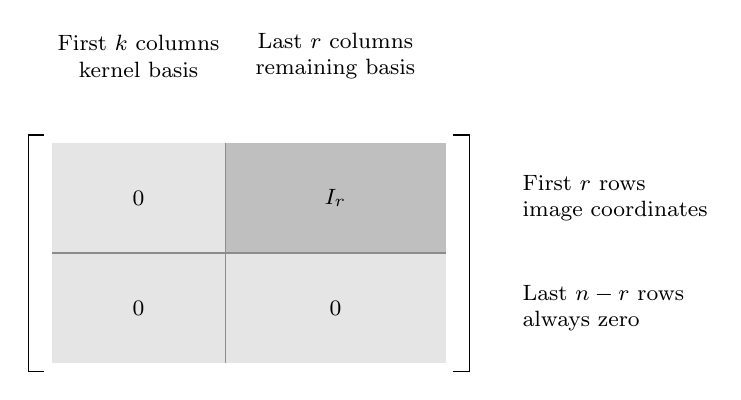
\begin{tikzpicture}[
  x=1mm,y=1mm,font=\footnotesize,line width=0.45pt,
  every node/.style={inner sep=2pt},
  group label/.style={align=center},
  row label/.style={anchor=west,align=left}
]
  \node[group label] at (11,11)
    {First \(k\) columns\\kernel basis};
  \node[group label] at (36,11)
    {Last \(r\) columns\\remaining basis};

  % Leave a gap between the labels and the matrix brackets.
  \fill[black!10] (0,0) rectangle (22,-28);
  \fill[black!25] (22,0) rectangle (50,-14);
  \fill[black!10] (22,-14) rectangle (50,-28);
  \draw[black!45] (22,0) -- (22,-28);
  \draw[black!45] (0,-14) -- (50,-14);
  \draw (-1,1) -- (-3,1) -- (-3,-29) -- (-1,-29);
  \draw (51,1) -- (53,1) -- (53,-29) -- (51,-29);

  \node at (11,-7) {\(0\)};
  \node at (36,-7) {\(I_r\)};
  \node at (11,-21) {\(0\)};
  \node at (36,-21) {\(0\)};

  \node[row label] at (59,-7)
    {First \(r\) rows\\image coordinates};
  \node[row label] at (59,-21)
    {Last \(n-r\) rows\\always zero};
\end{tikzpicture}

  \caption[Matrix adapted to the kernel and image.]{Schematic of the adapted matrix \(D\).
    The identity block carries the \(r\) surviving coordinates.
    Block sizes are indicated by the labels, not drawn to scale.
    A coordinate group disappears from \(D\) when its dimension is zero.}
  \label{fig:linear-algebra-i:adapted-basis-blocks}
\end{figure}

\begin{samepage}
To see its action, split an input coordinate column into
\(u\in\mathbb F^k\) and \(t\in\mathbb F^r\). Then
\[
  a=\begin{bmatrix}u\\t\end{bmatrix},
  \qquad
  Da=\begin{bmatrix}t\\0\end{bmatrix},
  \qquad 0\in\mathbb F^{n-r}.
\]
In other words, if \(v=Ea\), then
\(L(v)=\sum_{j=1}^r t^j f_j\).
\marginnote{%
  The identity block copies the surviving coefficients because
  \(f_j\) was chosen to equal \(L(e_{k+j})\).
  It does not assert that \(L\) is the identity map on \(V\).}
The \(k\) kernel coordinates \(u\) have no effect on the output.
This makes nullity \(k\) and rank \(r\) directly visible.
\par
\end{samepage}

\begin{example}
  For the standard bases of \(\R^m\) and \(\R^n\), the prescription
  \[
    L(e_1)=\cdots=L(e_k)=0,\qquad L(e_{k+j})=f_j\quad(1\leq j\leq r)
  \]
  gives the matrix \(D\) in
  \autoref{eq:linear-algebra-i:kernel-first-normal-form}.
  Here \(r=m-k\leq n\). Its nullity is \(k\) and its rank is \(r\).
  It is injective when \(k=0\), and surjective when \(n-r=0\).
\end{example}

% Source: MA-GY7033 Fall 2026 Homework 4.pdf, p. 1, Problem 3.
\begin{exercise}
  \label{ex:hw04:prescribed-kernel-and-image}
  \solutionlink{hw04:prescribed-kernel-and-image}
  Define the subspaces
  \[
    K=\operatorname{span}\{(1,1,0),(0,1,1)\}\subseteq\R^3
  \]
  and
  \[
    S=\operatorname{span}\{(1,2,1)\}\subseteq\R^3.
  \]
  Construct a linear map \(L:\R^3\to\R^3\) such that
  \[
    \ker L=K\qquad\text{and}\qquad\operatorname{im}L=S.
  \]
  \begin{enumerate}[(a)][2]
    \item Give an explicit formula for \(L(x,y,z)\).
    \item Write \(L\) as a matrix
    \item Prove that its kernel and image are exactly \(K\) and \(S\),
      rather than merely containing these subspaces.
    \item Verify rank-nullity for your map.
  \end{enumerate}
\end{exercise}


\subsection{Using the identity \(L(E)=FM\)}

% Source: September 24 slides 16--19. The author requested an explicit
% computational walkthrough of this identity on October 1, 2026.
The identity \(L(E)=FM\) is a recipe for finding the matrix of \(L\)
in the ordered bases \(E=[e_1,\ldots,e_m]\) and \(F=[f_1,\ldots,f_n]\).
Here
\[
  L(E)=[L(e_1),\ldots,L(e_m)]
\]
means applying \(L\) to each basis vector and placing the images in
columns. If \(M_j\) is the \(j\)-th column of \(M\), the corresponding
column of \(FM\) is
\[
  FM_j=f_1M^1_j+\cdots+f_nM^n_j.
\]
Thus \(L(E)=FM\) says that each column of \(M\) contains the
coefficients of \(L(e_j)\) in the basis \(F\).

To construct \(M\), proceed one column at a time.
\begin{enumerate}[(1)][1]
  \item Compute \(L(e_j)\), using the given formula for \(L\).
  \item Express this output as a linear combination of
    \(f_1,\ldots,f_n\). Equivalently, solve
    \(FM_j=L(e_j)\) for its coefficient column \(M_j\).
    The coefficients are unique because \(F\) is a basis.
  \item Place that coefficient column in position \(j\).
    Repeat in the order of \(E\), giving \(M=[M_1,\ldots,M_m]\).
\end{enumerate}
The resulting matrix has \(n\) rows and \(m\) columns.
Multiplying \(FM\) should reproduce all the computed images in \(L(E)\);
this is a direct check of the construction.

For a map between coordinate spaces, let \(C\) be its standard-basis
matrix, and write \(E\) and \(F\) as matrices whose columns are the
basis vectors in standard coordinates. Then \(L(E)=CE\), so
\[
  CE=FM,\qquad M=F^{-1}CE.
\]
The matrix \(F\) is invertible because its columns form a basis.
In practice, one can compute \(CE\) and solve \(FM=CE\) column by
column. The next example carries out the coefficient method directly.

\begin{example}
  \label{ex:linear-algebra-i:adapted-basis-matrix}
  Consider \(L:\R^3\to\R^2\) with standard-basis matrix
  \[
    C=\begin{bmatrix}1&2&3\\0&0&4\end{bmatrix}.
  \]
  Its kernel is
  \[
    \{(v^1,v^2,0):v^1+2v^2=0\},
  \]
  with basis \(\{(-2,1,0)\}\). Choose the domain and codomain bases
  \[
    E=[(-2,1,0),(0,1,0),(0,0,1)],
    \qquad F=[(2,0),(3,4)].
  \]
  As matrices of standard coordinates, these are
  \[
    E=\begin{bmatrix}-2&0&0\\1&1&0\\0&0&1\end{bmatrix},
    \qquad F=\begin{bmatrix}2&3\\0&4\end{bmatrix}.
  \]
  Applying \(C\) to the columns of \(E\) gives\marginnote{%
    Although \(L(e_2)=(2,0)\) in standard coordinates, it equals \(f_1\).
    Its column in \(M\) is therefore \((1,0)^T\), recording one copy
    of \(f_1\) and zero copies of \(f_2\).}
  \[
    \begin{aligned}
      L(e_1)&=(-2+2,0)=(0,0)=0f_1+0f_2,\\
      L(e_2)&=(2,0)=1f_1+0f_2,\\
      L(e_3)&=(3,4)=0f_1+1f_2.
    \end{aligned}
  \]
  The three coefficient columns are therefore
  \[
    M_1=\begin{bmatrix}0\\0\end{bmatrix},\qquad
    M_2=\begin{bmatrix}1\\0\end{bmatrix},\qquad
    M_3=\begin{bmatrix}0\\1\end{bmatrix}.
  \]
  Placing these columns in order gives\marginnote{%
    Here \(k=1\) and \(r=2\), so the adapted matrix has one zero column
    followed by \(I_2\). Since \(n=r=2\), there are no unused output
    coordinates and no lower block of zero rows.}
  \[
    M=[M_1,M_2,M_3]=\begin{bmatrix}0&1&0\\0&0&1\end{bmatrix}.
  \]
  To check \(L(E)=FM\), multiply
  \[
    \begin{aligned}
      FM
        &=\begin{bmatrix}2&3\\0&4\end{bmatrix}
          \begin{bmatrix}0&1&0\\0&0&1\end{bmatrix}\\
        &=\begin{bmatrix}0&2&3\\0&0&4\end{bmatrix}
          =[L(e_1),L(e_2),L(e_3)]=L(E).
    \end{aligned}
  \]
  Thus, for \(v=e_1a^1+e_2a^2+e_3a^3=Ea\),
  \[
    L(v)=f_1a^2+f_2a^3=FMa.
  \]
\end{example}

% Source: MA-GY7033 Fall 2026 Homework 4.pdf, p. 2, Problem 4.
\begin{exercise}
  \label{ex:hw04:adapted-bases}
  \solutionlink{hw04:adapted-bases}
  Let \(L:\R^3\to\R^2\) be defined by
  \[
    L(x,y,z)=(x+y+z,\;x+2y+3z).
  \]
  \begin{enumerate}[(a)][2]
    \item Find a basis for \(\ker L\).
    \item Extend this basis to an ordered basis \(E=(e_1,e_2,e_3)\)
      of \(\R^3\), with \(e_1\) spanning \(\ker L\).
    \item Choose an ordered basis \(F=(f_1,f_2)\) of \(\R^2\)
      such that
      \[
        L(e_2)=f_1,\qquad L(e_3)=f_2.
      \]
    \item Find the matrix \(M\) of \(L\) with respect to \(E\) and \(F\).
    \item Verify directly the identity
      \[
        L(E)=FM.
      \]
  \end{enumerate}
\end{exercise}


An alternative normal form places the identity block first.
If \(C\) represents a map \(\mathbb F^m\to\mathbb F^n\)
of rank \(r\), there are invertible matrices \(A\) and \(B\) such that
\[
  C=A
  \begin{bmatrix}
    I_r&0_{r\times(m-r)}\\
    0_{(n-r)\times r}&0_{(n-r)\times(m-r)}
  \end{bmatrix}
  B^{-1}.
\]
The displayed block order differs from the kernel-first form in
\autoref{eq:linear-algebra-i:kernel-first-normal-form}.
% The author's source states this factorization without its proof. Block
% sizes have been made explicit from the supplied domain, codomain, and rank.
